%----------------------------------------------------------------------------------------
%	METODE
%----------------------------------------------------------------------------------------
\section*{METODE PENELITIAN}

Penelitian yang dilakukan mengikuti kaidah pengembangan sistem \textit{prototyping}. Model \textit{prototyping} terdiri dari beberapa tahapan yaitu komunikasi (pengumpulan kebutuhan), perencanaan dan pemodelan cepat, pembuatan \textit{prototype}, pengembangan sistem serta pengiriman hasil dan umpan balik (\textit{deployment delivery} dan \textit{feedback} atau evaluasi) (\cite{Pressman2010}). Gambar \ref{fig:tahapan} menunjukan tahapan proses pada metode \textit{prototype}.

\begin{figure}[h!] % Gunakan \begin{figure*} untuk memasukkan Gambar
\centering
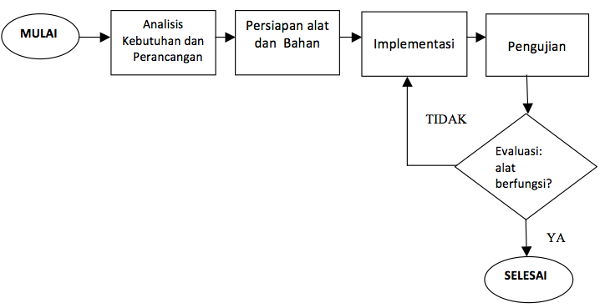
\includegraphics[width=200pt]{kolokium_contoh_gb1.png}
\caption{Tahapan proses penelitian (\cite{Pressman2010})}
\label{fig:tahapan}
\end{figure}

\subsection*{Komunikasi}

Tahapan ini mendefinisikan kebutuhan keseluruhan sistem. Mengidentifikasi proses bisnis, jenis ternak dan pakan yang akan digunakan. Jenis ternak yang digunakan adalah ternak ruminansia. Ternak ruminansia adalah jenis hewan ternak yang mampu mencerna pakan hijauan yang berserat tinggi dan pakan konsentrat seperti sapi, kerbau, domba dan kambing. Jenis pakan sendiri terbagi menjadi sumber protein, sumber energi, sumber vitamin dan sumber mineral yang dikelompokkan menjadi dua jenis yaitu pakan hijauan dan pakan konsentrat (Hidayat dan Mukhlas 2015). Sedangkan ransum diartikan sebagai satu atau beberapa jenis pakan yang diberikan kepada hewan ternak dan dapat memenuhi zat gizi yang dibutuhkan ternak untuk berbagai fungsi tubuhnya (Muhammad et al. 2014). Pada tahapan ini akan dilakukan komunikasi antara peternak dan pengembang untuk kebutuhan \textit{transfer knowledge} dari pakar kepada pengembang.

\subsection*{Perencanaan Cepat}

Menurut \citeauthor{Pressman2010} (\cite*{Pressman2010}) setelah tahap komunikasi dilakukan, selanjutnya adalah tahap perancangan dan pemodelan sistem. Perancangan dan pemodelan yang dibuat disesuaikan dengan kebutuhan sistem yang telah didefinisikan pada tahap komunikasi. Perancangan dapat dideskripsikan melalui tabel kebutuhan fungsional sistem, digram use case dan diagram antar tabel. 

\subsection*{Pemodelan Cepat}

Pemodelan yang dilakukan pada tahapan ini adalah pemodelan \textit{linier programming} dengan metode simpleks pada penghitungan formulasi. \textit{Linier programming} merupakan metode matematika dalam mengalokasikan sumber daya yang terbatas untuk mencapai suatu tujuan seperti memaksimumkan keuntungan atau meminimumkan biaya. \textit{Linier programming} banyak diterapkan dalam masalah ekonomi, industri, militer dan sosial. Penggunaannya dalam formulasi ransum dapat digunakan untuk mendapatkan harga seminimal mungkin (Wirdasari 2009). \textit{Linier programming} dapat digunakan untuk menentukan campuran makanan ternak dengan efisien. \textit{Linier programming} mampu menentukan kombinasi terbaik antar pakan yang tersedia. Persamaan matematis \textit{linier programming} bertujuan untuk meminimumkan dapat dilihat pada persamaan dibawah ini.\\

Fungsi tujuan : \\
Z = c_{1}x_{1}+c_{2}x_{2}+...+C_{n}x_{n}\\

Dengan fungsi kendala:\\
a_{11}x_{11} + a_{21}x_{21} + ... + a_{n1}x_{n1} \leq  b1\\
a_{12}x_{12} + a_{22}x_{22} + ... + a_{n2}x_{n2} \leq  b2\\
..\\
..\\
a_{1m1}x_{1m} + a_{2m}x_{2m} + ... + a_{nm}x_{nm} \leq  bm\\
x_{1},x_{2}, ... , x_{n} \geq 0\\

\\
keterangan:\\
Z	=	fungsi tujuan yaitu nilai total harga minimum dari pembuatan ransum\\
x	=	nilai penggunaan bahan pakan dalam bentuk persentase\\
c	=	koefisien harga tiap pilihan bahan pakan\\
a	=	koefisien nilai komposisi nutrien yang terkandung dalam suatu bahan pakan\\
b	=	nilai pembatas berupa nilai minimum dan maksimum nutrien yang dibutuhkan oleh unggas serta nilai minimum dan maksimum penggunaan bahan pakan\\
m	=	jumlah pembatas\\
n	=	jumlah bahan pakan yang digunakan dalam komposisi pembuatan ransum.\\

Tiap pakan memiliki kandungan nutrisi dan harga yang berbeda sehingga linier programming memformulasikan ransum hingga mendapatkan ransum dengan harga paling minimum. Hasil dari formulasi tergantung pada nilai kebutuhan nutrisi ternak, jumlah pakan dan jenis pakan yang digunakan pada ransum. Harga akhir juga dipengaruhi oleh komposisi nutrisi dari bahan pakan yang dipilih dan unit harga dari tiap bahan pakan yang digunakan. Meminimumkan harga pakan menjadi fungsi tujuan dari pemodelan ini, dengan kendala-kendala kandungan nutrisi dari setiap bahan pakan dan kebutuhan nutrisi jenis ruminansia yang diinputkan.
Menurut \citeauthor{Hidayat2013} (\cite*{Hidayat2013}) \textit{linier programming }memiliki syarat, yaitu:
\begin{enumerate}[noitemsep] 
	\item[a] \textit{Linier programming }harus memiliki fungsi tujuan (\textit{objective function}) berupa garis lurus dengan persamaan fungsi Z atau f(Z), c adalah \textit{cost coefficient}
	\item[b] Harus ada kendala (\textit{constraints}), yang dinyatakan garis lurus, dimana a = koefisien input-output dan b = jumlah sumber daya yang tersedia. 
	\item[c] Nilai X adalah positif atau sama dengan nol. Tidak boleh ada nilai X yang negatif.
\end{enumerate}
\textit{Linier programming }dapat digunakan untuk menentukan campuran makanan ternak yang efisien, praktis dan relatif mudah digunakan. Sesuai definisi, \textit{linier programming} adalah suatu teknik untuk menentukan kombinasi terbaik diantara pakan yang tersedia, yang mempunyai mempunyai kandungan nutrisi dan harga yang berbeda, dalam rangka untuk mendapatkan ransum dengan harga serendah mungkin. Hasil dari formulasi tersebut tergantung pada nilai yang digunakan untuk : 1) kandungan nutrisi dan spesifikasi lainnya yang diperlukan dalam ransum, 2) komposisi nutrisi dari bahan pakan yang dipilih, dan 3) unit harga dari tiap bahan pakan yang digunakan. Meminimumkan harga pakan akan menjadi fungsi tujuan dari model program linear, dengan kendala-kendala kandungan nutrisi dari setiap bahan pakan dengan sumber daya yang telah ditentukan (\cite{Hidayat2013}).

\subsection*{Pembuatan \textit{Prototype}}

Membangun \textit{prototyping} dengan mengimplementasikan hasil perancangan pada tahap sebelumnya. \textit{Prototyping} harus mampu menggambarkan sistem yang akan dikembangkan. Komponen yang digunakan dalam pembuatan \textit{prototype} harus berdasarkan hasil perancangan dari tahap perancangan dan pemodelan.

\subsection*{\textit{Deployment Delivery} dan \textit{Feedback}}

\textit{Prototype }yang telah dikembangkan dilakukan evaluasi oleh pengguna yang memahami alur proses formulasi ransum. Evaluasi bertujuan untuk memastikan alur proses pada sistem yang telah dikembangkan sesuai dengan kebutuhan pengguna dan tidak ada tahapan atau hasil penghitungan yang salah. Evaluasi tidak hanya dilakukan pada kebutuhan fungsional sistem, tetapi juga terhadap hasil akhir formulasi yang akan dibandingkan dengan program WinFeed. Nilai akurasi dari hasil perbandingan dihitung menggunakan \textit{Mean Avarage Percentage Error} MAPE. Pengujian ini bertujuan untuk mengetahui nilai rata-rata kesalahan dari hasil formulasi. Menurut Suryaningrum dan Wijaya (2015) MAPE dihitung dengan menggunakan kesalahan absolut pada tiap prediksi dibagi dengan nilai aktual hasil formulasi. MAPE merupakan pengukuran kesalahan yang menghitung ukuran presentase penyimpangan antara data aktual dengan data prediksi. Nilai MAPE dapat dihitung dengan persamaan berikut:\\

\\
MAE = \dfrac{100\%}{n} (\dfrac{\sum(|Xt-Yt|)}{Xt})
\\

\\
keterangan:\\
Xt	=	hasil formulasi pada aplikasi X percobaan ke-t\\
Yt	=	hasil formulasi pada alikasi Y percobaan ke-t\\
n	=	jumlah percobaan\\

Jika hasil evaluasi sudah sesuai dengan kebutuhan pengguna dan memiliki nilai penghitungan formulasi yang sesuai maka pengembangan selesai dilakukan, jika evaluasi belum sesuai kebutuhan maka \textit{prototype} diperbaiki dengan melakukan iterasi selanjutnya. 
